% YZM 5110 Multimodal Learning, Project 1 -- research report (IEEE conference format)
% Build: pdflatex report (twice, so the citation numbers resolve)
% Needs IEEEtran.cls (TeX Live package texlive-publishers). The bibliography is embedded: no bibtex run needed.
\documentclass[conference]{IEEEtran}

\usepackage[T1]{fontenc}
\usepackage[utf8]{inputenc}
\usepackage{lmodern}
\usepackage{microtype}
\usepackage{graphicx}
\usepackage{booktabs}
\usepackage{tabularx}
\usepackage{longtable}
\usepackage{array}
\usepackage{amsmath,amssymb}
\usepackage{url}
\usepackage{tikz}
\usetikzlibrary{positioning,arrows.meta}
\usepackage[hidelinks]{hyperref}

\sloppy
\emergencystretch=2em
\newcommand{\code}[1]{\texttt{\detokenize{#1}}}

\begin{document}
\pagestyle{plain}

\title{Robustness of MAMEX to Corrupted Text\\
in Cold-Start Recommendation}

\author{\IEEEauthorblockN{Hatice Sebla Karabunar}
\IEEEauthorblockA{Artificial Intelligence and Data Engineering Department\\
Y{\i}ld{\i}z Technical University\\
Repository: \url{https://github.com/karabunar/multimodal-coldstart-recsys-robustness}}}

\maketitle
\thispagestyle{plain}

\begin{abstract}
MAMEX is a cold-start recommender witch gate gives weight to an image expert and text expert. I ask what the gate do when an item's text is present but misleading, and what a fix depend on. On Amazon Baby the released code reproduce Recall@20 at 0.0776 against 0.0771 published. It doesn't reproduce Recall@10, and I couldn't found the cause. I corrupt the text of 40\% of cold items at test time. Recall@20 drop by 14\% on three seeds and 12\% on fifteen. The gate is nearly constant and don't react much. A training-free repair blend in the text of the visually nearest warm items where an item's text look wrong. I call this Gated Neighbour Blend (GNB). It recover about 85\% of loss, beats random-neighbour and permuted controls in 12 of 15 seeds, and holds on five unused seeds with predictions fixed beforehand. The repair works only when cold items' features was in the training losses. When they are left out, detection falls from AUROC 0.999 to 0.72 and the gain fall from $+0.0078$ to $+0.0004$. Three remedies I try fail or reach about a fifth of the gain. A simple baseline that drops suspect text and rank by image, the Image-Only Fallback, recovers 79\% of the loss.
\end{abstract}

\begin{IEEEkeywords}
cold-start recommendation, multimodal recommendation, mixture of experts, robustness, reproducibility
\end{IEEEkeywords}

%====================================================================
\section{Research Question, Scope, Contributions}

\textbf{Question.} MAMEX~\cite{nguyen2025mamex} builds a cold item's embedding by letting a gate to weight an image expert and a text expert. Suppose the item's text is present but misleading, for example clickbait. Do the gate keep trusting it? And can parameter-free image--text agreement signal reduce damage without hurting clean accuracy?

\textbf{Scope.} I use Amazon Baby item cold-start split. It have 7,050 items, of which 1,410 is cold, and 19,442 training users. Text is corrupted at test time only, on 40\% of cold items. Most of corruption is done on embeddings, and one check use real titles. I use three seeds first, fifteen for main comparison and five more for confirmation. I build Amazon Sports myself from LATTICE files and use it only as robustness check. Other cold-start models are out of scope.

\textbf{Contributions.} (1)~A condition. A training-free repair of corrupted cold-item text work only when cold items' features was in the alignment loss during training. Three inductive remedies fails or reach about a fifth of gain. (2)~Controls. VGR's gain is mostly reached by controls that ignore image, and an Image-Only Fallback recover 79\% of the loss against 85\% for the repair. (3)~A stress-test protocol, VGR, and neighbour-text repair with controls. (4)~A measured reproduction, where Rec@10 gap stays open. (5)~A confirmation run on five unused seeds with predictions fixed beforehand. (6)~A tested codebase.

Every number is measured here or come from a cited paper, and I mark an inference as my reading. Only confirmation run was fully specified before it ran, and repository history cannot show the order of writing. Other analyses are exploratory, and I applied no correction for multiple comparisons.

\begin{table}[!t]
\centering\footnotesize
\caption{Main results at a glance (Recall@20 unless stated, details in Section~\ref{sec:results}).}
\label{tab:glance}
\begin{tabularx}{\columnwidth}{@{}>{\raggedright\arraybackslash}p{2.4cm}X@{}}
\toprule
Result & Value \\
\midrule
Reproduction & 0.0776 against 0.0771 published. Recall@10 is 0.0486 (mean of 15 seeds; 0.0487 on the first 3) against 0.0512, and 0 of 15 seeds reach it. \\
Corruption & $-14\%$ on 3 seeds, $-12\%$ on 15 seeds, and the gate is nearly unchanged. \\
VGR & $+0.0026$ over 15 seeds. About two thirds of it is reached by controls that ignore the image. \\
GNB repair & $+0.0078$ over 15 seeds, positive in 15/15 and above both controls in 12/15. \\
GNB, cold items left out of training & $+0.0004$, with detection AUROC 0.999 $\to$ 0.721. \\
Confirmation & 6 of 6 frozen predictions hold on 5 unused seeds. \\
\bottomrule
\end{tabularx}
\end{table}

%====================================================================
\section{Literature Search and Critical Synthesis}
\label{sec:lit}

\textbf{Procedure.} I ran one web query for each of VBPR, MMGCN, CLCRec, MoToRec and MAMEX, and two topic queries. DGMRec came up as follow-up. I added MILK~\cite{bai2024milk} because MAMEX README acknowledge it. This is targeted selection and not a systematic review. I read all seven papers in full and check each matrix row against text. Detailed comparison table is in Appendix~\ref{app:matrix} (Table~\ref{tab:matrix}). It have one row per paper: the five required papers plus DGMRec and MILK as supporting work. Each row has seven fields: question and contribution, modalities and assumptions, mechanism and objective, data and protocol, baselines and evidence, resources and reproducibility, and limitations and connections. Every entry is marked as reported by authors or as my interpretation. This section gives only short version, and numbers and protocol details sits in the table.

\textbf{The papers.} VBPR~\cite{he2016vbpr} adds image features to BPR-MF and report gains for items with little feedback. MMGCN~\cite{wei2019mmgcn} builds one user-item graph per modality, so its items must already be in graph. CLCRec~\cite{wei2021clcrec} and MoToRec~\cite{liu2026motorec} targets cold start. CLCRec align content and collaborative signals. MoToRec argues that noisy continuous embeddings cause ``semantic fog'' and use discrete tokens instead. MAMEX~\cite{nguyen2025mamex} is the paper I reproduce. It keep continuous features and let a gate weight the modalities. DGMRec~\cite{kim2025dgmrec} and MILK~\cite{bai2024milk} handles missing modalities, which is the problem closest to mine.

\textbf{Synthesis.}
\begin{enumerate}
\item \emph{Shared pipeline, incomparable numbers.} All of them uses frozen pre-extracted features. ``Cold'' means fewer than 5 positives in VBPR, fewer than 10 in MoToRec, and none in CLCRec and MAMEX. MMGCN and MoToRec splits interactions at random. MoToRec reports a Baby R@20 of 0.0347 for its cold group and MAMEX reports 0.0771, but they use different protocols.
\item \emph{The nearest remedies treat a failing modality as absent.} MILK mean-fills it and train over Dirichlet-weighted fusion environments. DGMRec generates it. Both works at training time, while VGR and my repair works on a trained model. In their setting the text is absent and in mine it is misleading, so I make no numerical comparison.
\item \emph{Content helps, and text is the likely shortcut.} Content help items with little or no history. VBPR reports a Women cold-start AUC of 0.6813 against 0.5281 for BPR-MF. MAMEX's ablation show both modalities beating either one alone. In that ablation text beat vision on Amazon, so text is the natural signal for a gate to lean on. This is my inference from the ablation, which the paper show only as a figure.
\item \emph{Evidence is thin where it matters for me.} CLCRec reports single runs without variance. MILK reports a mean of five runs, also without variance in text I read. VBPR states no seeds or significance tests. MAMEX leaves batch size, epochs and embedding size unstated. MAMEX and DGMRec have no limitations section. MoToRec and MMGCN call their features noisy or irrelevant, but neither corrupt an input to test it.
\item \emph{Reproducibility varies.} MMGCN, CLCRec, MAMEX, DGMRec and MILK has public code or say they release it. VBPR give no link in the text I read. MoToRec states no code and no hardware. MILK and DGMRec gives their optimiser, embedding size and early stopping. MAMEX does not. So I use MAMEX repository's settings and list my deviations in Section~\ref{sec:repro}.
\item \emph{Narrower than ``nobody tested this''.} None of the seven papers test a modality that is present but misleading. A later search found closer work. Li~\cite{li2026trustworthy}, a preprint, gives corrupted item features to another item and evaluate warm backbones on random splits. Its fix is an offline rectification step before training. Zhong \emph{et al.}~\cite{zhong2024mirror} trains a flat-minima strategy against input noise on warm backbones. I test misleading text on the gate of cold-start model at test time and with controls. I didn't compare with these methods.
\end{enumerate}

\textbf{Consequences for this project.} I reproduce MAMEX's complete cold-start setting, because there a new item has no interactions at all. VBPR and MoToRec define cold start more loosely, so their numbers are no reference. MAMEX is only evaluated on clean features and has no limitations section, so it's open what its gate do when the text disagrees with the image. That is what I test. MILK and DGMRec fix missing modalities during training. I wanted a fix that work on a model that is already trained. The settings differ, so I treat these papers as context and not as baselines (Section~\ref{sec:improve}).

%====================================================================
\section{The Method: MAMEX as Implemented}

I read the model code and check it against the paper's equations. Fig.~\ref{fig:arch} shows the model and additions of this work.
\begin{itemize}
\item Frozen, L2-normalised image and text features each passes through a mixture-of-experts layer with 4 linear experts, of which top 2 are used. This give a 128-d embedding per modality and a load-balancing loss.
\item A fusion gate gives $[w_v, w_t]$. It is an MLP with ReLU and dropout and a softmax over two outputs. The item embedding is $w_v e_{\text{img}} + w_t e_{\text{txt}}$. There is no item-id embedding, so an item's embedding depend on its features alone. User embeddings are free parameters.
\item The loss have four parts: BPR plus L2, an alignment MSE between item and modality embeddings, an expert balance loss, and a KL term that keep the mean gate near uniform. Cold items are scored from their features alone.
\item \emph{Against the paper.} I compared the code with arXiv 2508.08042v1, Eqs.~3--11. The structure match, with two differences. Eq.~5 describes a sparse softmax gate, but the code use an MLP with an ordinary softmax. The alignment MSE in the code is smaller than the paper's squared L2 norm by embedding size of 128. The paper don't say which scale its weight $\lambda_1$ uses.
\end{itemize}

\begin{figure*}[!t]
\centering
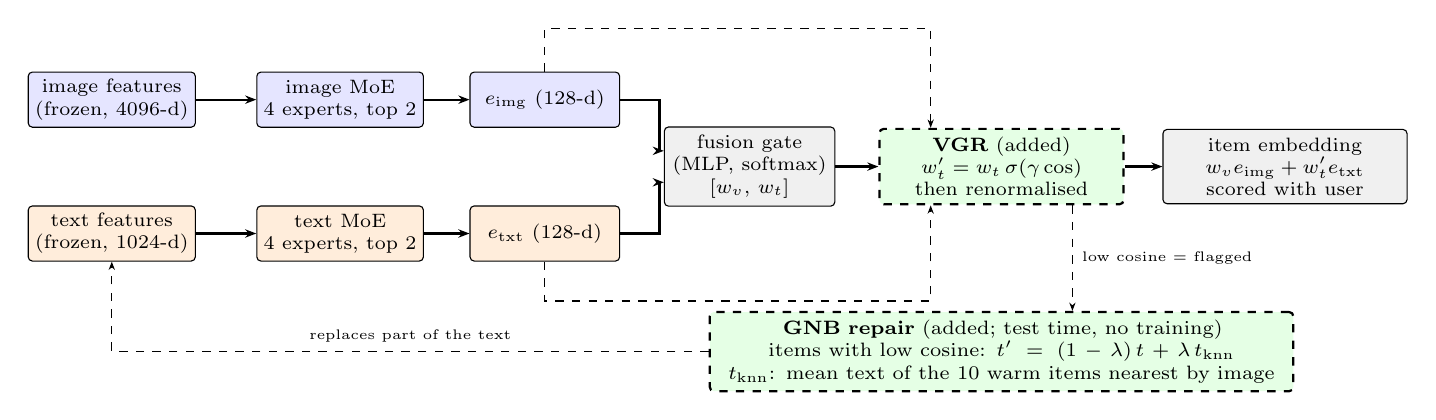
\begin{tikzpicture}[font=\scriptsize, x=1cm, y=1cm,
  feat/.style={draw, rounded corners=1.5pt, align=center, inner sep=2.5pt, minimum width=1.9cm, minimum height=0.7cm},
  imgc/.style={fill=blue!10},
  txtc/.style={fill=orange!14},
  orig/.style={draw, rounded corners=1.5pt, align=center, inner sep=3pt, fill=gray!12, minimum height=0.9cm},
  ours/.style={draw, dashed, thick, rounded corners=1.5pt, align=center, inner sep=3pt, fill=green!10, minimum height=0.9cm},
  arr/.style={-{Stealth[length=4pt]}, thick},
  thin arr/.style={-{Stealth[length=3pt]}, dashed}]
% image and text paths
\node[feat, imgc] (fi) at (1.0,1.0) {image features\\(frozen, 4096-d)};
\node[feat, txtc] (ft) at (1.0,-0.7) {text features\\(frozen, 1024-d)};
\node[feat, imgc] (mi) at (3.9,1.0) {image MoE\\4 experts, top 2};
\node[feat, txtc] (mt) at (3.9,-0.7) {text MoE\\4 experts, top 2};
\node[feat, imgc] (ei) at (6.5,1.0) {$e_{\mathrm{img}}$ (128-d)};
\node[feat, txtc] (et) at (6.5,-0.7) {$e_{\mathrm{txt}}$ (128-d)};
\draw[arr] (fi) -- (mi); \draw[arr] (mi) -- (ei);
\draw[arr] (ft) -- (mt); \draw[arr] (mt) -- (et);
% gate, VGR, item embedding
\node[orig] (gate) at (9.1,0.15) {fusion gate\\(MLP, softmax)\\$[w_v,\,w_t]$};
\node[ours, minimum width=3.1cm] (vgr) at (12.3,0.15) {\textbf{VGR} (added)\\$w_t'=w_t\,\sigma(\gamma\cos)$\\then renormalised};
\node[orig, minimum width=3.1cm] (item) at (15.9,0.15) {item embedding\\$w_v e_{\mathrm{img}}+w_t' e_{\mathrm{txt}}$\\scored with user};
\draw[arr] (ei.east) -- ++(0.5,0) |- ([yshift=0.2cm]gate.west);
\draw[arr] (et.east) -- ++(0.5,0) |- ([yshift=-0.2cm]gate.west);
\draw[arr] (gate) -- (vgr);
\draw[arr] (vgr) -- (item);
% cosine inputs to VGR
\draw[thin arr] (ei.north) -- ++(0,0.55) -| ([xshift=-0.9cm]vgr.north);
\draw[thin arr] (et.south) -- ++(0,-0.5) -| ([xshift=-0.9cm]vgr.south);
% GNB repair
\node[ours, text width=7.2cm] (m3) at (12.3,-2.2) {\textbf{GNB repair} (added; test time, no training)\\items with low cosine: $t'=(1-\lambda)\,t+\lambda\,t_{\mathrm{knn}}$\\$t_{\mathrm{knn}}$: mean text of the 10 warm items nearest by image};
\draw[thin arr] ([xshift=0.9cm]vgr.south) -- node[right, font=\tiny]{low cosine = flagged} ([xshift=0.9cm]m3.north);
\draw[thin arr] (m3.west) -- node[above, font=\tiny]{replaces part of the text} (1.0,-2.2) -- (ft.south);
\end{tikzpicture}
\caption{MAMEX as used here and where the additions act. Grey boxes are the model as released and dashed green boxes are additions of this work. Blue is the image path and orange the text path. VGR and GNB act on a trained model at evaluation time. The cosine is $\cos(e_{\mathrm{img}},e_{\mathrm{txt}})$ of the two 128-d embeddings, shown by the dashed inputs.}
\label{fig:arch}
\end{figure*}

%====================================================================
\section{Reproduction Target, Implementation, Deviations}
\label{sec:repro}

\textbf{Target.} The published values comes from Table~1 of the paper and I keep them apart from my measurements. They are Rec@10 0.0512, Rec@20 0.0771, NDCG@10 0.0292 and NDCG@20 0.0363. \textbf{Implementation.} The upstream code, commit \code{88a932e}, was restructured into a package, with characterisation tests before change and unit and end-to-end tests after it. Claude Code wrote this under my direction (see Use of AI Tools); I specified structure and check the results. Training and evaluation logic are unchanged. The additions is test-time corruption, VGR, the repairs with controls, $\gamma$ selection on validation data and an evaluation report. Reused components are listed in \code{docs/reused\_components.md}.

\textbf{Deviation 1, feature source.} The released data carry LATTICE's features~\cite{zhang2021lattice} and not CLIP as paper states. The Baby files published by LATTICE's authors is identical to the distributed ones, with 7,050 rows and a maximum absolute difference of 0.0. My data folder is byte-identical to the authors' \code{processed\_data\_baby.zip} in 30 of 30 files by SHA-256. I couldn't trace the preprocessing. The authors answered a public issue on their repository (issue \#2) by pointing to MMSRec code and the raw Amazon data. No preprocessing script for Baby features is provided. All results uses the released features. I do not offer the feature source as cause of the Rec@10 gap, because Rec@20 and NDCG@20 match and no experiment varied the features.

\textbf{Other deviations.} The paper omit batch size, epochs, embedding size and hardware, so I use the repository defaults. These is batch 2,048, 128-d embeddings, up to 1,000 epochs and early stopping at 200, with best epoch chosen on clean validation NDCG@10. The first seeds are 2025 to 2027, and 2025 is upstream default. I didn't pick any seed by looking at results. I wrote the reproduction criterion after I seen the baseline. It says a metric is questioned if published value lies outside the seed range.

%====================================================================
\section{Proposed Improvement and Rationale}
\label{sec:improve}

\textbf{VGR.} After the gate I set $w_t' = w_t \cdot \sigma(\gamma \cos(e_{\text{img}}, e_{\text{txt}}))$ and renormalise $[w_v, w_t']$. The cosine use the 128-d post-MoE embeddings and have no gradient. VGR has no learned parameters, so it can be switched on or off on same clean-trained checkpoint. My rationale, written before the results, is that alignment pull the two embeddings together on clean data. A low cosine then signal text that disagrees with the image. One cost was known in advance, which is that $\sigma<1$ also down-weights clean text.

\textbf{Training-free repair.} VGR lowers a suspect text's weight but put nothing in its place. I therefore replace part of text by $t_{\mathrm{knn}}$, the mean unit text of the ten warm items nearest by image cosine. I name the versions myself. They are not methods from literature, and the code and result files call them \code{m1} and \code{m3}.
\begin{itemize}
\item \emph{Neighbour Blend (NB)} blend $t_{\mathrm{knn}}$ into every cold item, $t'=(1-\lambda)t+\lambda t_{\mathrm{knn}}$, without any detection.
\item \emph{Gated Neighbour Blend (GNB)} blend it only where VGR's cosine $c_i$ is low. The weight is $\lambda_i=\lambda_{\max}\sigma(g(Q_q-c_i))$, where $Q_q$ is the $q$-quantile of the cosines over cold items.
\item \emph{Image-Only Fallback (IOF)} is baseline. For the same flagged items it drop the text and ranks them by image alone.
\end{itemize}
An earlier variant gated by the agreement between $t$ and $t_{\mathrm{knn}}$ was dropped, because its score add nothing over a permuted score. Controls are random warm neighbours and permuted scores. All parameters is chosen on noisy validation data and never on test set. These are $\gamma$, $\lambda$, $\lambda_{\max}$, $q$ and $g$.

\textbf{Hypotheses.} I wrote each of the five hypotheses together with the result that would falsify it, and Table~\ref{tab:hyp} list them. Supporting analyses are in \code{docs/hypotheses.md} and mechanism probes is in Appendix~\ref{app:probes}.

\begin{table*}[!t]
\centering\footnotesize
\caption{The five hypotheses and their outcomes. ``Supported'' means all stated predictions held. Thresholds are in the scripts and in \code{docs/hypotheses.md}.}
\label{tab:hyp}
\renewcommand{\arraystretch}{1.0}
\begin{tabularx}{\textwidth}{@{}>{\raggedright\arraybackslash}p{3.7cm}>{\raggedright\arraybackslash}p{5.3cm}>{\raggedright\arraybackslash}X@{}}
\toprule
Research question & Prediction & Outcome \\
\midrule
1. Does the gate keep trusting corrupted text? & Corruption lowers accuracy and the gate do not move away from text. & Supported. Recall@20 $-14\%$, $w_t$ 0.550 $\to$ 0.563, gate nearly constant across items. \\
2. How much do VGR and the neighbour-text repairs recover, and is it grounding or muting? & VGR recover part of the loss and needs the image. Image-guided repairs beat random-neighbour and permuted controls, and GNB beat the blind blend NB. & Partly. VGR recover 27--38\% of the loss, latency +5.6\% (limit missed), and controls recover about two thirds of its gain. Repairs beats controls and GNB is above NB by $+0.0019$ over fifteen seeds. On a second dataset the ranking hold with a smaller effect. \\
3. Do the gains depend on the transductive setting, and do they replicate? & The cosine and the repairs survive when cold items are left out of training losses, an inductive repair exists, and main claims replicate on five unused seeds. & No for the first two (AUROC 0.72, GNB $+0.0004$ against $+0.0078$, ridge detector AUROC 0.57). Yes for replication, six of six frozen predictions (Section~\ref{sec:confirm}). \\
4. Why does the gate trust text? (exploratory) & The preference come from the training interactions, not from the item's content. & Supported on a noise-augmented model, through routes other than those first guessed, on two to three seeds (Appendix~\ref{app:probes}). \\
5. Is a better detector enough to make the repair work when the cold items were not seen in training? & A contrastive detector trained on warm items find the corrupted items better (AUROC at least 0.72) and lifts GNB's inductive gain to at least $+0.0015$. & Partly. AUROC 0.87, but GNB $+0.0014$, a fall of 0.0045 in clean Recall@20; the detector read image-text agreement (shuffled text 0.91) and miss Gaussian noise (0.51). \\
\bottomrule
\end{tabularx}
\end{table*}

%====================================================================
\section{Experimental Design}
\label{sec:design}

\begin{itemize}
\item \textbf{Data and setting.} I use Baby item cold-start split as distributed. Cold items has no training interactions. Their features still passes through the model at every step and enter the alignment and balance losses, but not BPR, as in upstream code. The setting is therefore transductive. Validation and test holds 705 cold items each, and candidates are all 1,410 cold items.
\item \textbf{Noise.} Corruption happen at test time only. Training and validation stays clean, so the clean control is exact. In the main hashtag noise a corrupted item's unit text vector is mixed with one of 5 shared clickbait prototypes, drawn from warm items, with weight 0.8. I also use shuffle, which give an item another item's text, and Gaussian noise. The rate is 0.4, which is 564 of 1,410 items. Noise is simulated on embeddings, and the same seed give the same mask in every mode.
\item \textbf{Conditions and metrics.} I compare clean, stress test, VGR on noisy and on clean text, two image-blind VGR controls, and the repairs. $\gamma\in\{1,2,4,8,16\}$ is chosen by NDCG@10 on noisy validation data with a different mask, and the epoch also use validation data only. Headline metrics are Recall@20 and NDCG@20 as mean $\pm$ sample std, with per-seed paired differences and bootstrap intervals over test users. With $n=3$ I ran no significance test.
\item \textbf{Environment.} One RTX A4000, about 19 min per run. PyTorch 2.9.1 is pinned and reproduce the saved baselines bit for bit. The later system PyTorch 2.14.1 do not, as Appendix~\ref{app:record} explains.
\end{itemize}

%====================================================================
\section{Results, Controls, Uncertainty, Failure Analysis}
\label{sec:results}

Test split, cold items, hashtag noise at 0.4, mean over seeds 2025--2027 unless stated.

\subsection{Reproduction}

\begin{table}[!t]
\centering\footnotesize
\caption{Published vs measured clean baseline.}
\label{tab:repro}
\begin{tabular}{@{}lcccc@{}}
\toprule
 & Rec@10 & Rec@20 & NDCG@10 & NDCG@20 \\
\midrule
Published & 0.0512 & 0.0771 & 0.0292 & 0.0363 \\
Measured, 3 seeds & 0.0487 & 0.0776 & 0.0285 & 0.0365 \\
Std over seeds & 0.0023 & 0.0042 & 0.0017 & 0.0022 \\
\bottomrule
\end{tabular}
\end{table}

Rec@20, NDCG@10 and NDCG@20 lies inside the seed range and within 0.001 of the mean. Rec@10 is 0.0025 above the mean, about one seed std of 0.0023. Ten seeds gives $0.0488\pm0.0004$ s.e. and fifteen seeds a mean of 0.0486, and none reach 0.0512. I try four diagnostics, with rules written first, and none closed the gap. The paper's three alignment-loss scales gave 0.0500 at best. Validation-based epoch rules gives 0.0482 to 0.0491. An epoch chosen with the test set gave 0.0502, which is diagnostic only. Ranking among the 705 test items only raise every metric by 53 to 59\%, so that protocol is excluded. I couldn't identify the cause of the gap and didn't pursue it further.

\subsection{Stress test and VGR}

\begin{figure*}[!t]
\centering
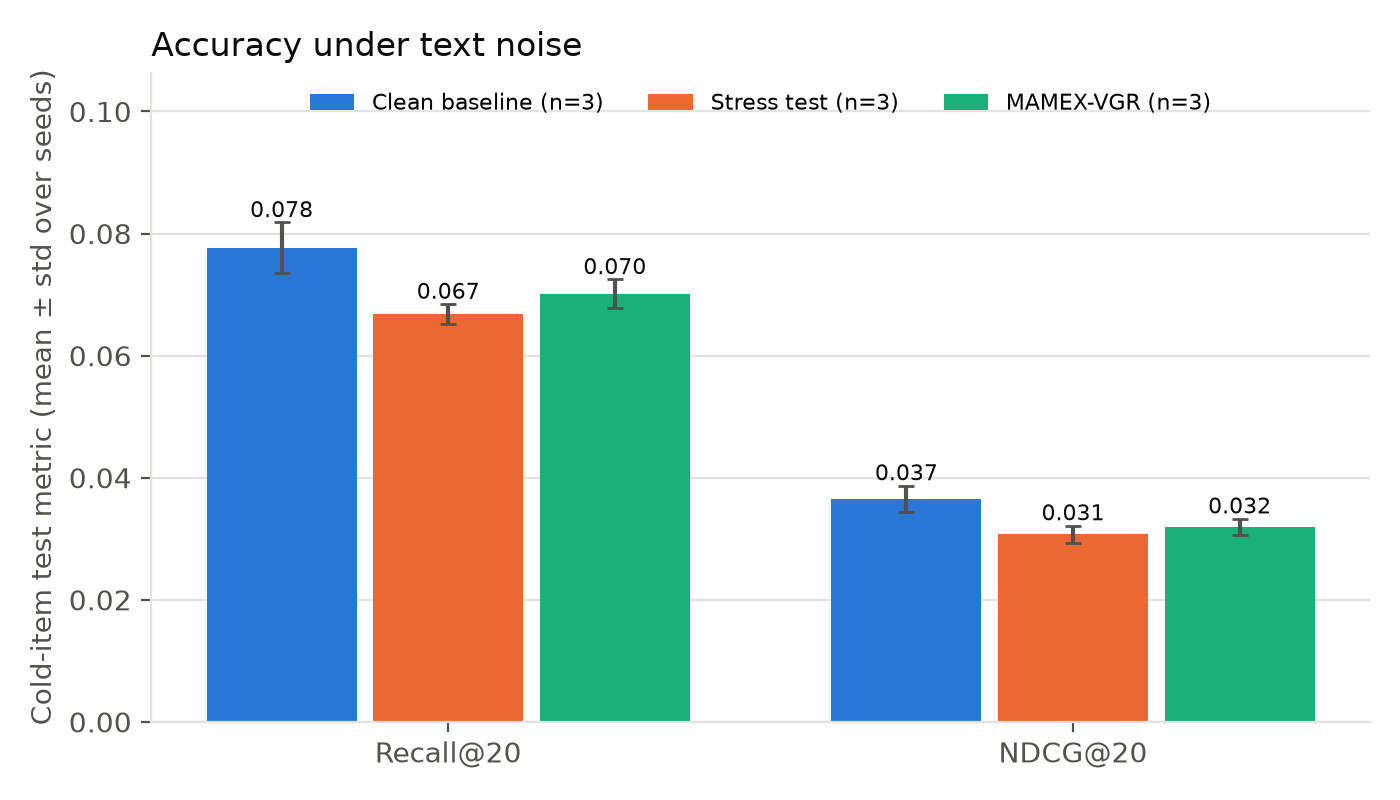
\includegraphics[width=0.48\textwidth]{fig/accuracy_comparison.png}\hfill
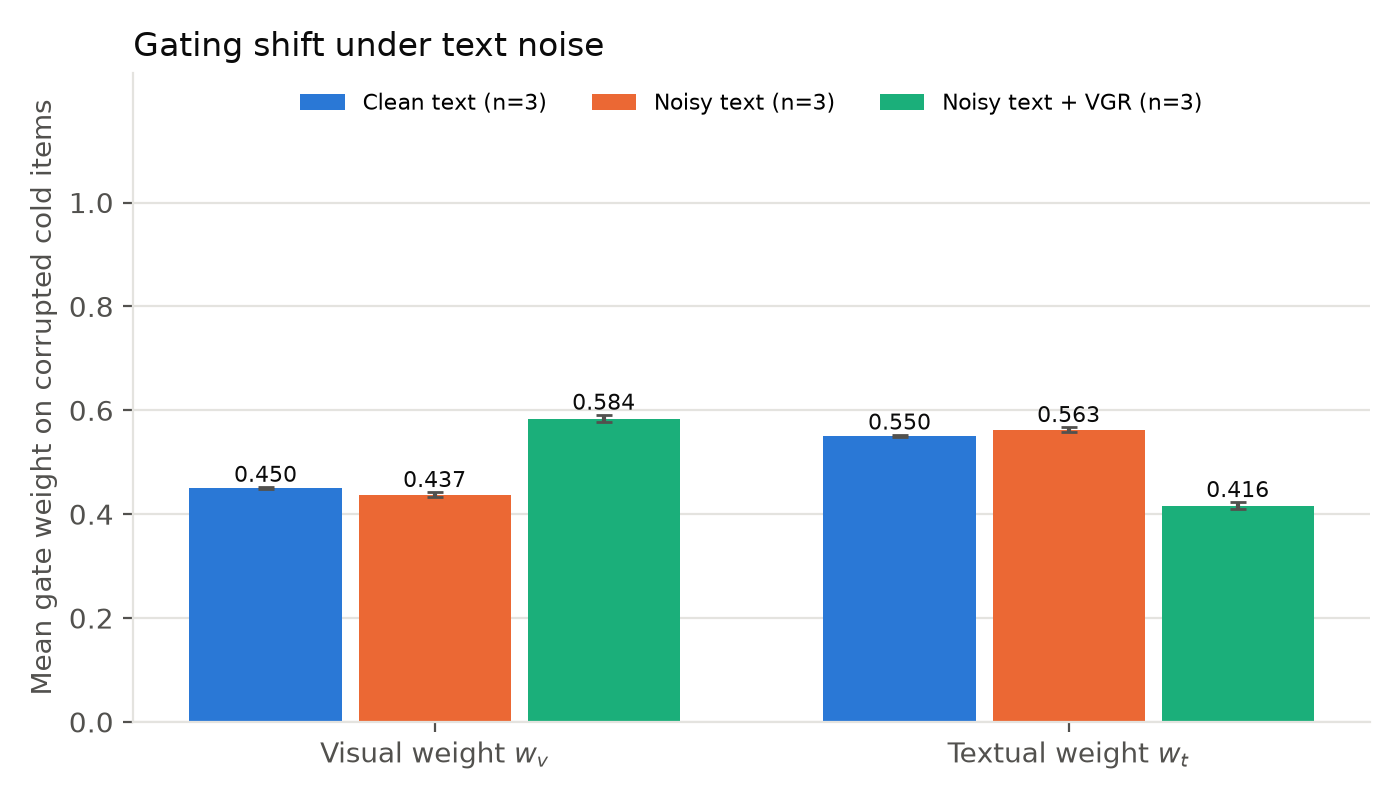
\includegraphics[width=0.48\textwidth]{fig/gating_weight_shift.png}
\caption{Left, accuracy under text noise. Right, mean gate weights on the corrupted cold items. Hashtag noise at 0.4, mean $\pm$ std over the first three seeds.}
\label{fig:stress}
\end{figure*}

\textbf{Hypothesis 1.} Corruption lower Recall@20 from 0.0776 to 0.0668, a fall of 14\%, and NDCG@20 from 0.0365 to 0.0307. On corrupted items $w_t$ goes from 0.550 to 0.563, so the gate don't move away from text (Fig.~\ref{fig:stress}). Over fifteen seeds the std of $w_t$ across cold items is only 0.050, and balance loss keep the mean near 0.5. So the gate is close to a fixed share, and the lack of a shift is not surprising.

\textbf{Hypothesis 2.} Noisy VGR beat noisy in 3/3 seeds with $+0.0033$ Recall@20, which is 27 to 38\% of the loss, and it move $w_t$ to 0.416. Clean VGR change Recall@20 by $-0.0004$. It also slow the forward pass by 5.6\%, above the 5\% limit I set in advance. Controls that ignore the image, a shuffled cosine and a constant factor, recovers about two thirds of VGR's gain. When they act among the cold items only, on fifteen seeds, VGR exceed them by just $+0.0010$ and $+0.0011$. The grounding-specific part is therefore about 8\% of the loss. A paired bootstrap over 10,474 test users give noisy minus clean $-0.0109$ [$-0.0129,-0.0087$] and VGR minus noisy $+0.0033$ [$+0.0024,+0.0044$]. The selected $\gamma$ was the grid minimum. I didn't chose it from a post hoc test-set sweep.

\subsection{Training-free repair}

\begin{table}[!htb]
\centering\caption{Recall@20, hashtag 0.4, seeds 2025--2027, gain over the unrepaired model (seeds with a positive gain).}
\label{tab:repair}
\small\setlength{\tabcolsep}{3pt}
\begin{tabular}{@{}>{\raggedright\arraybackslash}p{3.3cm}ccc@{}}
\hline
Method & noisy text & gain & clean text \\
\hline
Unrepaired & 0.0668 & n/a & 0.0776 \\
VGR & 0.0701 & $+0.0033$ (3/3) & 0.0773 \\
NB (blind blend) & 0.0746 & $+0.0078$ (3/3) & 0.0769 \\
GNB (cosine-gated) & 0.0761 & $+0.0094$ (3/3) & 0.0792 \\
GNB, random neighbours & 0.0644 & $-0.0023$ (0/3) & 0.0721 \\
GNB, permuted cosine & 0.0724 & $+0.0056$ (3/3) & 0.0794 \\
Oracle (true mask) & 0.0735 & $+0.0068$ (3/3) & 0.0776 \\
\hline
\end{tabular}
\end{table}

The image guidance is what help. Both repairs beats their random-neighbour controls in 3/3 seeds. The agreement-gated variant that I dropped (Section~\ref{sec:improve}) lose to a permuted score. Its AUROC is 0.51 to 0.71, against 0.999 for VGR's cosine. NB gain $+0.0078$ at a clean cost of only $-0.0007$. GNB gain $+0.0094$, about 86\% of the 0.0109 lost, and 96\% with VGR. It is above NB and above both controls in all three seeds. The ``oracle'' that repair exactly the corrupted items is not an upper bound, since GNB and even NB beat it. Part of gain is general smoothing. Blending \emph{clean} cold text with neighbour text at $\lambda=0.25$ raises Recall@20 from 0.0770 to 0.0788 in 15/15 seeds. Under subtler noise the cosine still find the corrupted items, with AUROC 0.991 and 0.995, but GNB is at least NB in only 1 of 5 seeds. I also run nine settings, with hashtag, shuffle and Gaussian noise at rates 0.2, 0.4 and 0.6. GNB beats unrepaired model and VGR in all nine and keep 99 to 116\% of its gain when validation noise is mismatched. It is at least NB in only five of nine. Building the repair cost 0.6 s once (\code{results/tables.md}).

\subsection{Fifteen seeds, second dataset, Image-Only Fallback}

\begin{table}[!htb]
\centering\caption{Recall@20, hashtag 0.4: unrepaired score and mean gains. Baby has fifteen seeds (2025--2039) and Sports three seeds (my split).}
\label{tab:seeds}
\scriptsize\setlength{\tabcolsep}{2pt}
\begin{tabular}{@{}lcccccc@{}}
\hline
 & unrep. & VGR & NB & GNB & GNB+VGR & GNB$-$NB \\
\hline
Baby, 15 seeds & 0.0677 & $+.0026$ & $+.0059$ & $+.0078$ & $+.0084$ & $+.0019$ \\
Sports, 3 seeds & 0.0775 & $+.0018$ & $+.0023$ & $+.0068$ & $+.0065$ & $+.0046$ \\
\hline
\end{tabular}
\end{table}
\begin{figure*}[!t]
\centering
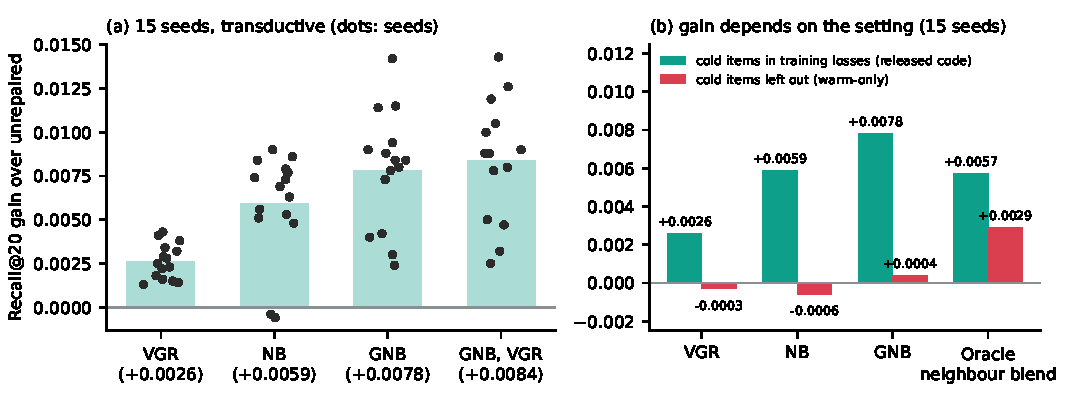
\includegraphics[width=0.92\textwidth]{fig/repair_gains.pdf}
\caption{Recall@20 gains over the unrepaired model, hashtag noise at 0.4. (a) The 15-seed grid, with the mean as a bar and each seed as a dot. (b) The same gains with the cold items inside and outside the training losses.}
\label{fig:repair}
\end{figure*}

GNB beat the unrepaired model in 15 of 15 seeds. It is at least as good as NB in 12 of 15 and beat both of its controls in 12 of 15 (Table~\ref{tab:seeds} and Fig.~\ref{fig:repair}). GNB minus NB have a mean of $+0.0019$ with std 0.0028, and a paired bootstrap interval over seeds of $[+0.0006,+0.0033]$. The lower end is close to zero and one seed carry part of the mean, which is $+0.0014$ without seed 2031. So GNB has a small advantage over the blind blend. On the first five seeds GNB recover about 85\% of the loss, and GNB followed by VGR about 93\%. On Sports, which I built myself with 35,598 users, 18,357 items and 3,671 cold items, all five predictions holds. GNB recovers only about 38\% of the loss there, against 85\% on Baby.

\textbf{Image-Only Fallback,} a baseline added after other results. For the same flagged items it drop the text, with weight 0, and rank them by image alone. Over fifteen seeds it recover 79\% of the loss, against 85\% for GNB and 64\% for NB. GNB is above it by only $+0.0005$ Recall@20, with s.e. 0.0005 and 11 of 15 seeds, and NDCG@20 favour the fallback, 0.0349 against 0.0345. The difference is on clean input. The same rule lower clean Recall@20 from 0.0770 to 0.0742, while GNB gives 0.0786. GNB keep clean accuracy, but it do not beat ignoring the corrupted text (\code{results/rq2\_image\_only.md}).

\subsection{Confirmatory run on unused seeds}
\label{sec:confirm}
Seeds 2040 to 2044 was never used before. I evaluated them once, under rules and six predictions written beforehand, and all six holds. Mean Recall@20 is 0.0770 clean and 0.0671 noisy, a loss of 0.0099 in 5/5 seeds against a predicted 0.007 to 0.015. It is 0.0696 with VGR, 0.0737 with NB and 0.0762 with GNB. GNB beat noisy in 5/5 seeds and is at least NB in 4/5. VGR beat its shuffled-cosine control in 5/5 seeds, by $+0.0011$ on average, and the AUROC of the cosine is 0.9991. This replicate the main grid in transductive setting. It say nothing about the inductive one, which Section~\ref{sec:transductive} covers.

\subsection{Real clickbait and real item text}
\label{sec:clickbait}\label{sec:realtext}
\textbf{Real clickbait vectors.} As a stricter check I replace the hashtag prototypes with embeddings of 41 clickbait strings. I made them with the text encoder I identify for the distributed features, \code{roberta-large-nli-stsb-mean-tokens}. Its vectors retrieves an item's own catalogue text as the top match for 61\% of 3,443 items, so it support the choice but do not prove it. I wrote five predictions before the fifteen-seed runs and all five holds. The loss is 14.9\% against 12\% for hashtag noise, and the AUROC of cosine is 0.9992. GNB gain $+0.0102$ against $+0.0078$, and it beats the unrepaired model and both controls in 15/15 seeds.

\textbf{Real item text.} Here I applies the corruption to the text of real products and embed it again. Of the 698 cold items with a 2023 catalogue entry, 80\%, about 40\% of all cold items, gets a corrupted title. The corruption is either a clickbait string in front of the title, called wrap, or another item's title, called mismatch. Using the titles alone cost 0.0017 Recall@20 against the original features, 0.0753 against 0.0770.

\begin{table}[!htb]
\centering\caption{Corrupted real titles, embedded again. Recall@20 and gains over the unrepaired model, 15 seeds (clean-title reference 0.0753). Last row: seeds in which GNB beats the unrepaired model, the random-neighbour and the permuted control.}
\label{tab:realtext}
\begin{tabular}{lcc}
\toprule
 & Wrap & Mismatch \\
\midrule
Unrepaired & 0.0721 & 0.0665 \\
AUROC of VGR's cosine & 0.939 & 0.989 \\
VGR gain & $+0.0026$ & $+0.0046$ \\
NB gain & $+0.0047$ & $+0.0077$ \\
GNB gain & $+0.0017$ & $+0.0063$ \\
Image-Only Fallback gain & $+0.0038$ & $+0.0095$ \\
GNB wins (seeds of 15) & 11, 7, 12 & 15, 15, 14 \\
\bottomrule
\end{tabular}
\end{table}

Most predictions holds. Mismatch cost more than wrap, and on mismatch GNB beat the unrepaired model and both controls in at least 14 of 15 seeds. Two predictions misses on wrapped titles. The cosine find them at AUROC 0.939, where I expected 0.60 to 0.85, and GNB beat the unrepaired model in only 11 of 15 seeds. The ranking of the repairs do not carry over. The Image-Only Fallback and the blind blend NB both gains more than GNB. A breakdown show that the edge of NB come mainly from smoothing clean cold text, which GNB do not get because it flag too few clean items. GNB also flag too many items overall, with precision 0.79 and recall 0.98 to 1.0. Why the fallback gain more than GNB on the corrupted items themselves is still open. Corruption is synthetic text on real products and not corrupted listings found in the wild.

\subsection{Dependence on the transductive setting}
\label{sec:transductive}
In the released code the cold items' clean features goes through the model at every training step. They enter the alignment and balance losses. Everything above was measured in that setting. With \texttt{-{}-warm\_only\_aux 1} only warm items is embedded and regularised during training, and a test check that cold features then have no influence on a step. I wrote predictions first and ran fifteen seeds, shown in Table~\ref{tab:transductive}.

\begin{table}[!htb]
\centering\caption{Cold items in or out of the training losses (Recall@20, hashtag 0.4, fifteen seeds, GNB gain positive in 8 of 15 seeds when out).}
\label{tab:transductive}
\footnotesize\setlength{\tabcolsep}{3pt}
\begin{tabular}{@{}lcc@{}}
\hline
 & in (main) & out \\
\hline
Clean Recall@20 & 0.0770 & 0.0756 \\
Noisy, unrepaired & 0.0677 & 0.0664 \\
AUROC of VGR's cosine & 0.999 & 0.721 \\
VGR beats noisy (seeds) & 15/15 & 4/15 \\
VGR gain & $+0.0026$ & $-0.0003$ \\
NB gain & $+0.0059$ & $-0.0006$ \\
GNB gain & $+0.0078$ & $+0.0004$ \\
Oracle neighbour blend, gain & $+0.0057$ & $+0.0029$ \\
\hline
\end{tabular}
\end{table}

The loss from corruption is same in both settings, 0.0093 and 0.0092. What is lost is the ability to find corrupted items, and with it most of the repair. Perfect detection still recover $+0.0029$, but VGR's cosine finds the items only at AUROC 0.72. Two inductive remedies, with predictions written first, also fails. One use a ridge map from raw image to raw text features as detector, at AUROC 0.565. The other blend flagged text toward the mean warm text instead of neighbour text, and lose $-0.0012$ with VGR's cosine and $-0.0021$ with ridge detector.

\textbf{Hypothesis 5.} A third detector is a two-tower network trained with an InfoNCE loss on warm items only, on clean text and without knowledge of noise. Its prediction was committed before the runs, an AUROC of at least 0.72 and a GNB gain of at least $+0.0015$. It find the corrupted items at AUROC 0.868, against 0.721 for VGR's cosine, which is better than I expect. It reads image--text agreement and not the look of the hashtags, with AUROC 0.910 for shuffled text but 0.508 for Gaussian noise. The GNB gain rise only to $+0.0014$, with 9 of 15 seeds positive and an interval over seeds of $-0.0001$ to $+0.0028$. That is half of the oracle's gain, and the repair lower clean Recall@20 from 0.0757 to 0.0712. Detection is therefore not the only obstacle. The detector is cheap, with 2.75 million parameters, 5.3 to 5.7 s of CPU training and 36 ms to score the cold items. VGR and GNB is not shown to work for items that arrive after training.

%====================================================================
\section{Limitations, Conclusions, Unresolved Questions}

\textbf{Limitations.} The reproduction is close but not exact, since 0 of 15 seeds reaches the published Rec@10 and I didn't identify the cause. The noise is simulated on embeddings, and real-text checks use 41 strings and 698 titles corrupted by construction. Sports is my own construction. Early experiments uses three seeds, and the gap between GNB and NB is of the order of the seed std. GNB beat the Image-Only Fallback, which I add after the other results, by only $+0.0005$. Mechanism findings rest on two to three seeds and one noise family. Gains need the cold items in the alignment loss during training, so they are not inductive cold-start results.

\textbf{Conclusions.} The main outcome is conditional. The improvement work where the released setting let the model see cold items' features during training, and I couldn't make it work where it does not. The transductive part is replicated on five unused seeds and the inductive part is negative on fifteen. The gate keep trusting corrupted text. VGR is a modest fix, since about two thirds of its gain come from muting text. GNB recover about 85\% of the loss on Baby and about 38\% on Sports, and building it take 0.6 s. It beats random-neighbour and permuted controls in 12 of 15 seeds. On real titles the Image-Only Fallback and the blind blend gains more than GNB, so its advantage is mainly that it keep clean accuracy.

\textbf{Unresolved questions.} Three things is open. Do any repair work for items that arrive after training? What close the Rec@10 gap? Do the pattern hold with real corrupted listings, other models, and features other than LATTICE's? It is also open what the gate's trace of training interactions encode (Appendix~\ref{app:probes}). An inductive design would needs new training runs of about 19 minutes per seed. One option is an alignment that make neighbour text a better stand-in for unseen items. Another is a gate that take the agreement cosine as input. I left both out.

\textbf{Mistakes I corrected.}
\begin{itemize}
\item VGR was first applied during training too. I made it an evaluation-time switch before any reported result. I had also mark the latency check as passed although 5.6\% exceeded my 5\% limit, and I had call the oracle an upper bound. It is not one.
\item My claim that a rerun reproduce every number failed when the system PyTorch changed from 2.9.1 to 2.14.1. The claim now name the environment.
\item The shuffled and constant controls ran over the whole catalogue and not over the cold items. With the fix, VGR's gain from image grounding fall from $+0.0017$ to $+0.0010$.
\item The text say cold items ``never appear in training'', but they enters the alignment and balance losses. I had called the hypotheses pre-registered, but most was written after earlier results. And I had claim that no related work exist, which was too strong.
\end{itemize}


%====================================================================
% Bibliography is embedded so the build needs no .bib file.
\section*{Use of AI Tools}
I use Claude Code (Anthropic CLI, model Claude Sonnet 5.5) to write code. I chose the approach: a layered (DDD-style) structure and test-driven (TDD-style) development. Under my direction Claude Code wrote the package structure, the analysis scripts and the tests. I ran experiments and check the results. The design and evaluation of the contrastive detector, the real-text experiment and the decomposition analysis (why GNB trail NB on real titles) is my own work, as are the literature work, the report and the review; the AI only edit those. The AI also did debugging. I remain responsible for reading the sources, checking the citations, and defending conclusions. A separate one-page statement list the contributions.

\begin{thebibliography}{9}
\bibitem{nguyen2025mamex} V.-K. Nguyen, D.-H. Pham, H.-S. Nguyen, C.-V. T. Nguyen, H.-Q. Le, and D.-T. Le, ``{MAMEX}: Multi-modal adaptive mixture of experts for cold-start recommendation,'' in \emph{Proc. 34th ACM Int. Conf. Information and Knowledge Management (CIKM)}, 2025, pp. 5053--5057, doi:10.1145/3746252.3760837.
\bibitem{he2016vbpr} R. He and J. McAuley, ``{VBPR}: Visual Bayesian personalized ranking from implicit feedback,'' in \emph{Proc. AAAI Conf. Artificial Intelligence}, vol.~30, no.~1, 2016, pp. 144--150, doi:10.1609/aaai.v30i1.9973.
\bibitem{wei2019mmgcn} Y. Wei, X. Wang, L. Nie, X. He, R. Hong, and T.-S. Chua, ``{MMGCN}: Multi-modal graph convolution network for personalized recommendation of micro-video,'' in \emph{Proc. 27th ACM Int. Conf. Multimedia (MM)}, 2019, pp. 1437--1445, doi:10.1145/3343031.3351034.
\bibitem{wei2021clcrec} Y. Wei, X. Wang, Q. Li, L. Nie, Y. Li, X. Li, and T.-S. Chua, ``Contrastive learning for cold-start recommendation,'' in \emph{Proc. 29th ACM Int. Conf. Multimedia (MM)}, 2021, pp. 5382--5390, doi:10.1145/3474085.3475665.
\bibitem{liu2026motorec} J. Liu, Z. Zhang, and R. C. C. Cheung, ``{MoToRec}: Sparse-regularized multimodal tokenization for cold-start recommendation,'' in \emph{Proc. 40th AAAI Conf. Artificial Intelligence}, vol.~40, no.~18, 2026, pp. 15324--15332, doi:10.1609/aaai.v40i18.38558.
\bibitem{bai2024milk} H. Bai, L. Wu, M. Hou, M. Cai, Z. He, Y. Zhou, R. Hong, and M. Wang, ``Multimodality invariant learning for multimedia-based new item recommendation,'' in \emph{Proc. 47th Int. ACM SIGIR Conf. Research and Development in Information Retrieval}, 2024, doi:10.1145/3626772.3658596.
\bibitem{kim2025dgmrec} J. Kim, H. Kang, S. Kim, K. Kim, and C. Park, ``Disentangling and generating modalities for recommendation in missing modality scenarios,'' in \emph{Proc. 48th Int. ACM SIGIR Conf. Research and Development in Information Retrieval}, 2025, pp. 1820--1829, doi:10.1145/3726302.3729953.
\bibitem{mmsrec} K. Song, Q. Sun, C. Xu, K. Zheng and Y. Yang, ``Self-supervised multi-modal sequential recommendation,'' arXiv:2304.13277, 2023 (paper and README of \url{https://github.com/kz-song/MMSRec} read).
\bibitem{li2026trustworthy} Z. Li, ``Towards trustworthy multimodal recommendation,'' arXiv:2602.00730, 2026, preprint.
\bibitem{zhong2024mirror} S. Zhong, Z. Huang, D. Li, W. Wen, J. Qin, and L. Lin, ``Mirror gradient: Towards robust multimodal recommender systems via exploring flat local minima,'' in \emph{Proc. ACM Web Conf. (WWW)}, 2024, arXiv:2402.11262.
\bibitem{radford2021clip} A. Radford \emph{et al.}, ``Learning transferable visual models from natural language supervision,'' in \emph{Proc. 38th Int. Conf. Machine Learning (ICML)}, PMLR vol.~139, 2021, pp. 8748--8763.
\bibitem{zhang2021lattice} J. Zhang, Y. Zhu, Q. Liu, S. Wu, S. Wang, and L. Wang, ``Mining latent structures for multimedia recommendation,'' in \emph{Proc. 29th ACM Int. Conf. Multimedia (MM)}, 2021, pp. 3872--3880, doi:10.1145/3474085.3475259.
\end{thebibliography}

%====================================================================
\appendices

\section{Reproduction Record}
\label{app:record}

\textbf{Submitted version.} Tag \code{v1.0} of the repository on page 1, on branch \code{main}.

\textbf{Source.} Reproduced code: \url{https://github.com/L2R-UET/MAMEX}, commit \texttt{88a932eca821a5657b2b\allowbreak 7fc0b6445e4685f4dfab}. This repository (URL on page 1) restructure it; model, loss and training loop is unchanged except for two switches that defaults to off.

\textbf{Environment.} Linux 7.0.0; Python 3.13.9; PyTorch 2.9.1 (CUDA 12.8) pinned in a separate virtual environment, which reproduce the saved baselines of seeds 2025--2027 exactly (the system PyTorch 2.14.1+cu130 do not); Intel Core i9-12900K, 62 GB RAM, NVIDIA RTX A4000. Packages is pinned in the requirements file.

\textbf{Data.} Baby, item cold-start split as distributed by authors (\url{https://drive.google.com/file/d/1C-18Y84lMS5xsRGwKQYa9P0Tot-gxgYY/view}; no raw text, images or ASIN mapping). ASINs of the 7,050 items comes from aligning the interaction graph with the 2014 Baby 5-core reviews (\code{scripts/align\_items\_to\_asin.py}); the 2023 Amazon Baby Products catalogue (\code{meta\_Baby\_Products.jsonl}, not included) give titles for 3,443 items and is used by the real-text checks. SHA-256 hashes of the data files is in \code{docs/reproducibility.md}. Data is not redistributed; Amazon review data is for research under their own terms.


\textbf{Seeds and configuration.} Training seeds 2025--2027 (first experiments, Sports), 2025--2039 (fifteen-seed comparison). The corruption seed default to the training seed; the validation mask use the seed plus 10,000. Upstream defaults otherwise.

\textbf{Commands} (repository root; full list in \code{docs/reproducibility.md}):
{\raggedright\scriptsize\ttfamily
PYTHONPATH=src python -m pytest -q\ \ (no GPU)\\
./scripts/demo.sh\ \ (about 2 min)\\
DATA\_PATH=processed\_data\_baby/cold\\
\ \ SEEDS="2025 2026 2027" ./scripts/run\_experiments.sh\\
./scripts/run\_repair.sh\ \ (repairs)\\
SRC=<Sports files> ./scripts/run\_second\_dataset.sh\par}
Tables and figures comes from the reporting modules.

\textbf{Cost.} About 19 min per run alone; the first 54 result files takes about 42 hours of training with shared GPU, the later repair and second-dataset runs adds 40.1 hours. Checkpoints is not published.


\section{Exploratory Mechanism Probes}
\label{app:probes}

These probes asks why the gate prefers text on cold items in a model trained with corrupted warm items, a noise-augmented ablation and not the main model. I wrote them after earlier results, on two to three seeds and one augmentation design, and no main claim rest on them. Training on corrupted warm items at rate 0.4 lower noisy Recall@20 to 0.0568 from 0.0668, and the gate put $w_t=0.917$ on noisy cold text against 0.563 without augmentation. The preference is not explained by gate bias or expert-output norm, and it follow from an item having no training interactions. Warm items whose interactions was removed gets $w_t$ of 0.97, like cold items, while trained items gets 0.35. Swapping one image-output component between cold and warm items move $w_t$ by 0.18--0.42, against 0.001 for random directions. My reading is that the gate read a trace of the training interactions in the image expert's output (details in \code{docs/hypotheses.md}).

\clearpage
\onecolumn
\section{Literature Comparison Matrix}
\label{app:matrix}

[Authors]: reported by paper. [Interpretation]: my inference. Results is those reported by each paper, and cold-start definitions differs, so numbers are not comparable across rows.

\begingroup\centering\scriptsize\setlength{\tabcolsep}{2pt}
\renewcommand{\arraystretch}{1.0}
\begin{longtable}{@{}p{1.6cm}*{7}{>{\raggedright\arraybackslash}p{2.2cm}}@{}}
\caption{Literature comparison matrix.}\label{tab:matrix}\\
\toprule
Paper & Question \& contribution & Modalities \& assumptions & Mechanism \& objective & Data \& protocol & Baselines \& evidence & Resources \& reproducibility & Limitations \& connections \\
\midrule
\endfirsthead
\toprule
Paper & Question \& contribution & Modalities \& assumptions & Mechanism \& objective & Data \& protocol & Baselines \& evidence & Resources \& reproducibility & Limitations \& connections \\
\midrule
\endhead
\bottomrule
\endfoot
VBPR~\cite{he2016vbpr} & Can product-image appearance improve implicit-feedback ranking, including for items with little feedback? [Authors]: add visual factors to BPR-MF. & Image (4096-d CNN FC7, ImageNet-pretrained) and implicit feedback. Items needs only an image to be scored. Users with $<5$ positives dropped. & $\hat{x} = \alpha + \beta_u + \beta_i + \gamma_u^{\top}\gamma_i + \theta_u^{\top}(E f_i) + \beta'^{\top} f_i$; BPR-OPT; 20 factors, half visual. & Amazon Women, Men, Phones, Tradesy. One random item per user for val and test. Cold = test items with $<5$ training positives (not zero). AUC. & RAND, MP, IBR, MM-MF, BPR-MF; hyperparameters tuned on validation; no seeds or significance tests. Women cold-start AUC: VBPR 0.6813 vs BPR-MF 0.5281; Phones: VBPR 0.6056 below IBR 0.6319 [Authors]. & Desktop, 4 cores, 32 GB; about 3.5 h on Women. Code ``at publication time'', no link in text. & Single image per item; visual/latent split fixed 50/50; no component ablation. Image only. \\
\midrule
MMGCN~\cite{wei2019mmgcn} & Model modality-specific user preferences for micro-video recommendation. [Authors]: one user-item graph per modality with message passing. & Visual, acoustic, textual pre-extracted features. Items must already sit in interaction graph, so it is not a cold-item method [Interpretation]. & Per-modality GCN aggregation (mean or max) with combination layers and a shared user-ID embedding; representations is the sum of the modality-specific ones, scored by inner product; BPR loss with L2; SGD. & Tiktok 726,065 / Kwai 1,664,305 / MovieLens 1,239,508 interactions. Random 8:1:1 over interactions; each test pair ranked against 1000 unobserved videos; Precision, Recall, NDCG@10. & VBPR, ACF, GraphSAGE, NGCF. Recall gains over strongest baseline 15.59\% / 10.23\% / 8.76\% (Kwai / Tiktok / MovieLens) [Authors]. Multimodal beat each single modality; visual is most effective, text least on Kwai and Tiktok. & Authors states they release codes, parameters and baselines. & Random interaction split: no cold-item evaluation, no corrupted-modality test. Call the Kwai/Tiktok descriptions ``noisy, incomplete, and even irrelevant'' but run no corrupted-text test. \\
\midrule
CLCRec~\cite{wei2021clcrec} & Cold-start item embeddings from an information-theoretic view: maximize mutual information between content and collaborative signals. & Pre-extracted visual, acoustic, text features (ResNet, VGGish, Sentence2Vector); Amazon use 64-d visual only. Cold items scored from content encoder alone. & Contrastive U-I and R-E objectives, $\lambda L_{RE} + (1-\lambda) L_{UI}$; hybrid training swap in content features with probability $\rho$. & Movielens, Tiktok, Kwai, Amazon; cold items split 1:1 into val/test, warm items 8:1:1. Recall@10, NDCG@10. & DUIF, DropoutNet, MTPR, CB2CF, Heater; same 64-d embedding for all. Single runs, no variance. & Code and data released; hardware not stated. & Single runs without variance. No text-corruption test. \\
\midrule
MoToRec~\cite{liu2026motorec} & Argues that aligning noisy continuous multimodal embeddings cause ``semantic fog''; propose discrete semantic tokens. & Visual (BEiT), text (BGE), learnable ID embeddings. Cold = items with $<10$ training interactions. Deployment for new items not described [Authors' text]. & Sparsity-regularised RQ-VAE per modality, rarity weighting, LightGCN-based multi-source graph encoder; $L_{BPR}+L_{CL}+L_{RQ}+L_{reg}$. & Amazon Baby (19,445 users, 7,050 items), Sports, Clothing. Random 8:1:1 over interactions; cold group = test items with $<10$ training interactions. R, N@\{10,20\}. & MF-BPR, LightGCN, VBPR, MMGCN, LATTICE, FREEDOM, BM3, LGMRec and others, in MMRec; grid search only described for MoToRec [Interpretation: baseline tuning fairness unverifiable]. Baby R@20 0.1077; Baby cold-start R@20 0.0347 [Authors]. & Hardware and code not stated. & Cold-start differ from complete cold start (items still has some interactions). Claim noisy embeddings are a problem but do not corrupt inputs to test it. \\
\midrule
MAMEX~\cite{nguyen2025mamex} & Cold-start fusion fail because concatenation, averaging or fixed weights ignores modality relations; adaptive gating across modality experts. & CLIP image and text features [Authors]; no dimensions stated. Complete item cold start: all interactions of dev/test items removed. & Modality-specific MoE (linear experts, top-$k$) and sparse-softmax gate over $[z_{img}\Vert z_{text}]$; $L_{BPR}+\lambda_1 L_{align}+\lambda_2 L_{adapter}+\lambda_3 L_{fusion}+\lambda_4\lVert\Theta\rVert^2$. & Amazon Baby, Clothing, Sports; 8:1:1; Rec, NDCG@\{10,20\}. & MTPR, AlignRec, MetaEmbed, DropoutNet, CLCRec, GAR, MILK. Baby: Rec@20 0.0771, NDCG@20 0.0363 [Authors]. Modality ablation (figure only): text beat vision, both beats either alone. & Code public (\url{github.com/L2R-UET/MAMEX}); batch size, epochs, embedding size and hardware not stated. & No limitations section; future work list missing modalities. Clean features only; the gate's behaviour under corrupted text is untested. Direct target of this project. \\
\midrule
DGMRec~\cite{kim2025dgmrec} & Multimodal recommenders degrades when item modalities are missing, and filling in a global or nearest-neighbour mean do not prevent it [Authors]. Disentangle general and modality-specific features and generate the missing ones. & Image and text on Amazon (a CNN for images, SBERT for text [Authors]); TikTok add audio. Some or all modality features of an item is absent; present features are assumed correct [Interpretation]. & Autoencoder; general and specific encoders trained with two information-based losses; a missing modality is generated from the other modalities and from the modality preferences of the item's users; generated features refines the item-item graph. & Amazon Baby, Sports, Clothing and TikTok; 8:1:1; Recall, NDCG@\{20,50\}. Missing setting: a third of items misses 0, 1 or 2 modalities; new-item setting: 20\% of items only in test; missing ratios 0 to 80\%. & 5 CF models, 10 multimodal recommenders (VBPR, MMGCN, LATTICE, LGMRec, GUME and others) and 3 missing-modality-aware ones; best in missing and new-item settings; drop 10.2\% vs 15.1\% for the compared baseline at an 80\% missing ratio [Authors]. & Code public (\url{github.com/ptkjw1997/DGMRec}); Adam, embedding size 64, up to 1,000 epochs, early stopping 30, $\lambda_1,\lambda_2$ tuned in $\{1,\allowbreak 0.1,\allowbreak 0.01,\allowbreak 0.001\}$. & No limitations section. Handle absent modalities, not present but misleading ones; the injected features it criticise is shown to hurt, the closest it come to a corrupted input, but no corrupted-text test is run [Interpretation]. \\
\midrule
MILK~\cite{bai2024milk} & New-item recommendation when items misses a modality. [Authors]: invariant learning, so that the user's preference prediction do not change across modality-missing environments; cross-modality alignment plus cyclic mixup. & Visual and text on Baby and Clothing; TikTok adds audio. Pre-extracted features, extractor and dimensions not stated in the text read [Interpretation]. A missing modality is mean-filled; present features is assumed correct [Interpretation]. & Modality-specific extractors with alignment functions between modalities; fusion weights $\Theta_1\sim$ Dirichlet, $M$ cyclic shifts and an equal-weight environment; $L = E_e L_e + \beta\,\mathrm{Var}_e L_e + \lambda L_{align} + \lVert\Phi\rVert^2$, BPR inside each environment. & Amazon Baby (19,442 users; 5,640 train, 705 val, 705 test items), Clothing, TikTok. 20\% of items new. FTMT: full training, one modality missing at test; MTMT: 30\% of training items also misses one. Recall, NDCG@\{10,20\}. & DUIF, MICRO, DropoutNet, MTPR, Heater, CLCRec, CCFCRec, GAR, GoRec. Baby FTMT Rec@20 0.0628, NDCG@20 0.0277 (best baseline GoRec 0.0544, 0.0249); mean of five runs, no variance stated in the text read [Authors]. MAMEX list MILK at Rec@20 0.0730 on Baby, a different setting [Interpretation]. & PyTorch, 64-d, batch 2048, Adam 0.001, early stopping; code public (\url{github.com/HaoyueBai98/MILK}); hardware not stated. $\beta$ is tuned per dataset (1000 on Baby). & Absence, not misleading content, is tested. Same item split as MAMEX and as this project (705 val and 705 test items). MAMEX's README acknowledges MILK for foundational concepts. \\
\end{longtable}
\endgroup

\end{document}
